% This is a model template for the solutions in computational science. You can find a very useful documentation for LaTeX in Finnish at ftp://ftp.funet.fi/pub/TeX/CTAN/info/lshort/finnish/ or in English at ftp://ftp.funet.fi/pub/TeX/CTAN/info/lshort/english/. The section List of mathematical symbols in Chapter 3 is especially useful for the typesetting of mathematical formulas.

% Compile the document to PDF by command 'pdflatex model.tex' in the terminal. The command must be run twice for the references in the text to be correct.

\documentclass[a4paper,11pt]{article}
\usepackage[utf8]{inputenc}
% This includes letters such as � and �
\usepackage[T1]{fontenc}
% Use here 'Finnish' for Finnish hyphenation. You may have to compile the code twice after the change. 
\usepackage[english]{babel}
\usepackage{graphicx}
% Some math stuff
\usepackage{amsmath,amsfonts,amssymb,amsbsy,commath,booktabs,hyperref,dirtytalk}  
% This is just to include the urls
\usepackage{float,hyperref,caption,subcaption}
\usepackage[margin=2cm]{geometry}

\setlength{\parindent}{0mm}
\setlength{\parskip}{1.0\baselineskip}

\usepackage{listings}
\usepackage{color}
\usepackage{pdfpages}

\definecolor{dkgreen}{rgb}{0,0.6,0}
\definecolor{gray}{rgb}{0.5,0.5,0.5}
\definecolor{mauve}{rgb}{0.58,0,0.82}

\lstset{frame=tb,
	language=Python,
	aboveskip=3mm,
	belowskip=3mm,
	showstringspaces=false,
	columns=flexible,
	basicstyle={\tiny\ttfamily},
	numbers=none,
	numberstyle=\tiny\color{gray},
	keywordstyle=\color{blue},
	commentstyle=\color{dkgreen},
	stringstyle=\color{mauve},
	breaklines=true,
	breakatwhitespace=true,
	tabsize=4
}

\begin{document}

\title{Becs-114.1100 Computational Science -- exercise round 10} % Replace the exercise round number
\author{Kunal Ghosh, 546247} % Replace with your name and student number
\maketitle
\section{Solution 1}\label{prob1}
In this exercise, we are experimenting with the Ising model, a mathematical model of ferromagnetism given by Ernst Ising. The premise is that, each cell (site) of the L x L lattice is an atom the spin of which can be +ve or -ve ( we are simulating that by +1 and -1 states in the L x L matrix ).\\
Monte-carlo simulations are then used to simulate the change in energy and magnetization of the (simulated) ferro-magnet as the temperature changes.\\
From theoretical results we know that for temperatures below 2.265 the ferro-magnets equilibriate to either positive or negative magnetization. At temperatures above 2.265 ( eg. 3.5 in our case ) the object exhibits para-magnetism and is disordered at equilibrium.\\
Finally at the Critial temperature ( 2.265 in this case ) the ferro-magnet goes through phase transition from ferro-magnetism to para-magnetism and fluctuates between positive and negative magnetization staying constant at a particular magnetization for long periods of time.
\\\textbf{NOTE:} In the experiments below, run 0 through 6 have been executed with \\ seeds 5555,6000,7000,8000,9000,10000,11000 respectively.
\clearpage
\subsection{Checking ground state energy}
Setting all the spins to -1 we see that the ground state energy of a 32 x 32 Lattice is -2048.0 which is as expected.
\subsection{Estimating suitable equilibriation time}
Jugdging from the plots below and table in section 1.5.1\\
\textbf{Equlibriation time for T  = 2.1 :} around 500 MCS\\
\textbf{Equlibriation time for T  = 3.5 :} around 200 MCS\\
\begin{figure}[!htb]
    \begin{subfigure}[b]{0.5\textwidth}
    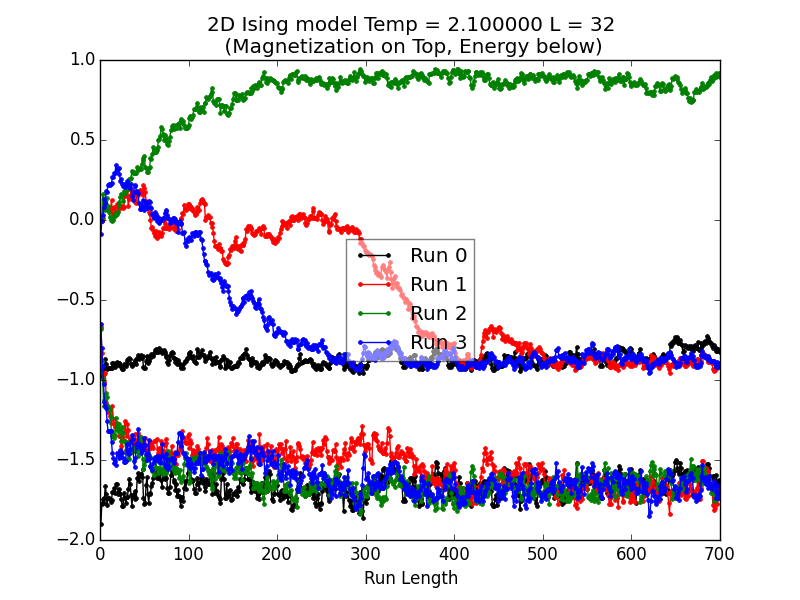
\includegraphics[scale=0.45]{new_pics/figure_both_2.png}
    \caption{T = 2.1}
	\label{fig:t2both}
\end{subfigure}
\begin{subfigure}[b]{0.5\textwidth}
    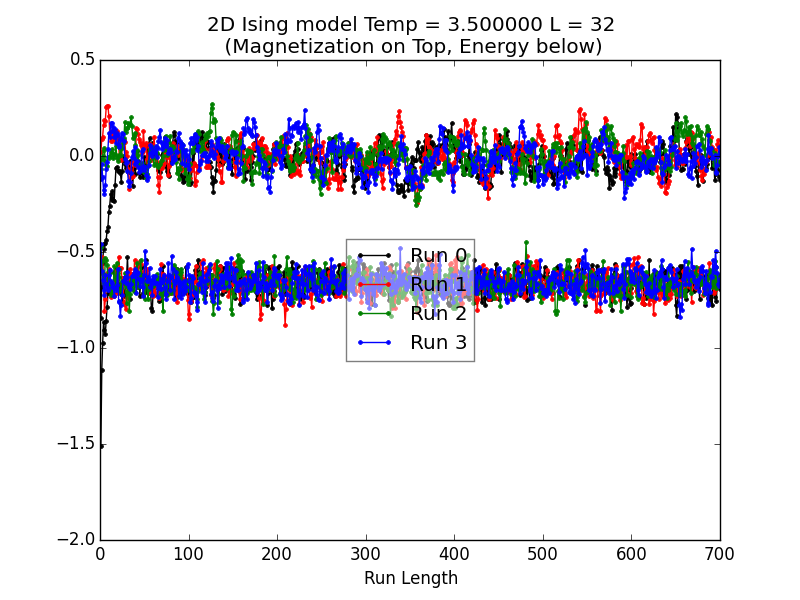
\includegraphics[scale=0.45]{new_pics/figure_both_35.png}
    \caption{T = 3.5}
	\label{fig:t3mag}
\end{subfigure}
\caption{Magnetization and energy plots at T = 2.1 and T = 3.5 for a 32 x 32 lattice. Time is measured on the X axis in MCS (Montecarlo Simulation) units.}
\end{figure}
\\
In the plots above, run 0 is started with the lattice having -1 at all the sites. This indicates the ground state where the enery is the least and the object is the most magnetized ( magnetization just above -1 ). This is the state we expect all the simulation runs to converge to at equilibrium. ( Some of the simulation runs converge to just below +1 which is another ground state which we have not plotted separately. )
\\
The plot to the left is of the object at T = 2.1 at which it is still ferro-magnetic hence some simulation runs assume positive or negative magnetization at equilibrium.\\
The plot to the right is of the object at T = 3.5 at which it assumes para-magnetism and it exhibits almost no magnetization (magnetization oscillating about 0, as observed in the plots).
\clearpage
\subsection{Simulation for T = 2.265}
\begin{figure}[!htb]
	\centering
    \includegraphics[scale=0.40]{pics/magnetization5000_2.png}
    \caption{Plot of the magnetization at T = 2.265. Simulation run for 50,000 MCS}
	\label{fig:5kmag}
\end{figure}
\textbf{What is happening ?}\\
T = 2.265 is the critical temperature at which the model undergoes \textbf{"phase transition"} and keeps fluctuating between magnetization = +1 and magnetization = -1 but staying constant at one magnetization for long periods of time (MCS).\\
\textbf{Effect of this behavior on time needed to perform measurements at this temperature ?}\\
At this temperature since the model keeps fluctuating (after long periods of stability) it causes any equilibrium calculation which considers magnetisation values only a few 100 MCS, falsely report that the model has reached equlibrium and fail to catch the flip in magnetization. Hence we must run the simulation for very a long time ( ~50,000 MCS in this case ) to figure out that the model is indeed going through phase transition and has not yet equilibriated.\\
Additionally, following the discussions on the topic \href{http://physics.stackexchange.com/q/5771}{[here]} and \href{http://physics.stackexchange.com/q/183398}{[here]} this phenomenon is called \textbf{"critical slowdown"} which causes the correlation length \href{Reference https://www.physicsforums.com/threads/what-is-correlation-length.733954/}{[ref]}(Time after which the deviations from the mean, stop being similar) to diverge. This means, we need to perform really long simulation runs to observe changes in correlation ( change in magnetization ). To avoid this, it is advisable to use either multiple simulation runs and average over them, to identify equilibrium, when using a local update scheme (as in this exercise) or use cluster update schemes of Montecarlo simulations. 

\clearpage
\subsection{Lattice Visualizations}
In the plots below we visualize the lattice after the simulations have reached equilibrium. Blue patches indicate magnetization of -1 and Red patches indicate magnetization of +1.
\subsubsection{T = 2.1}
\begin{figure}[!htb]
    \begin{subfigure}[b]{0.5\textwidth}
        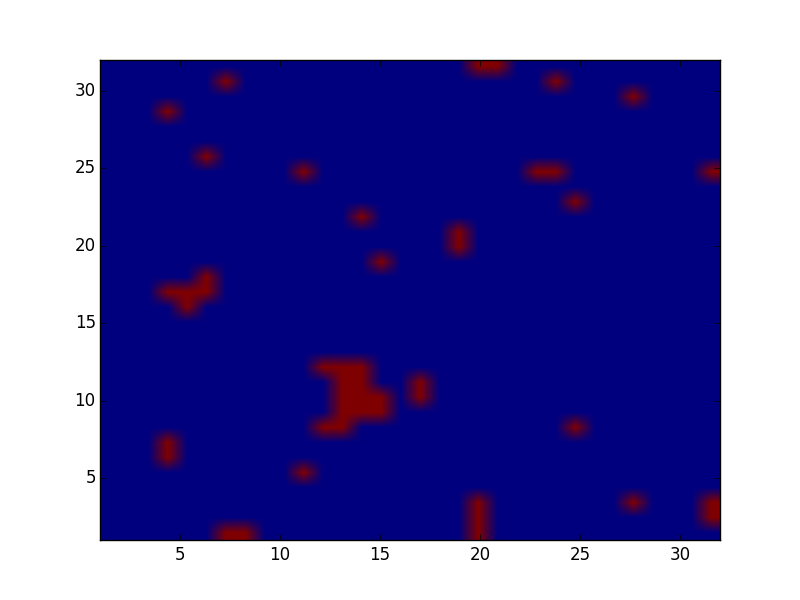
\includegraphics[scale=0.40]{2_run_0.png}
        \caption{Run 0, lattice initialized to -1, and simulations converges to just above -1}
	    \label{fig:lat2_0}
    \end{subfigure}
    \begin{subfigure}[b]{0.5\textwidth}
        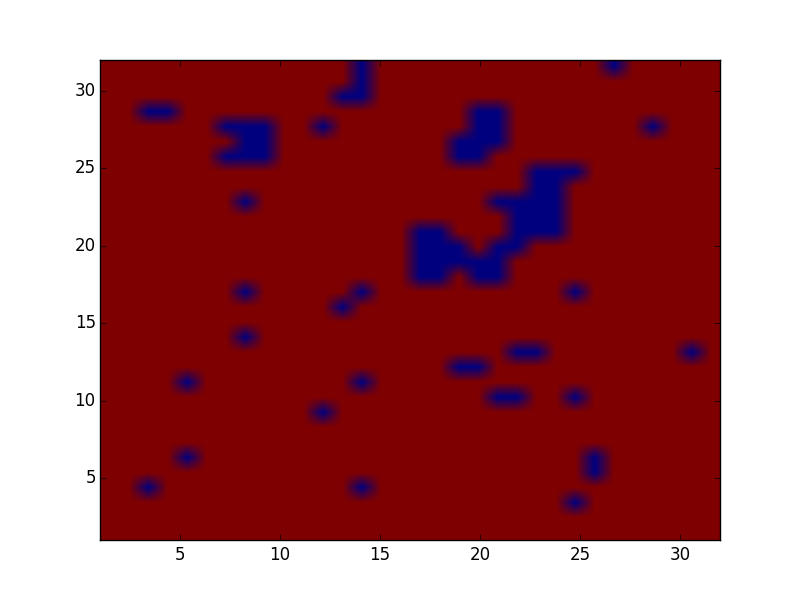
\includegraphics[scale=0.40]{2_run_2.png}
        \caption{Run 2, Random Initialization, converges to just below 1.0}
	    \label{fig:lat2_2}
    \end{subfigure}
    \begin{subfigure}[b]{0.5\textwidth}
        \centering
        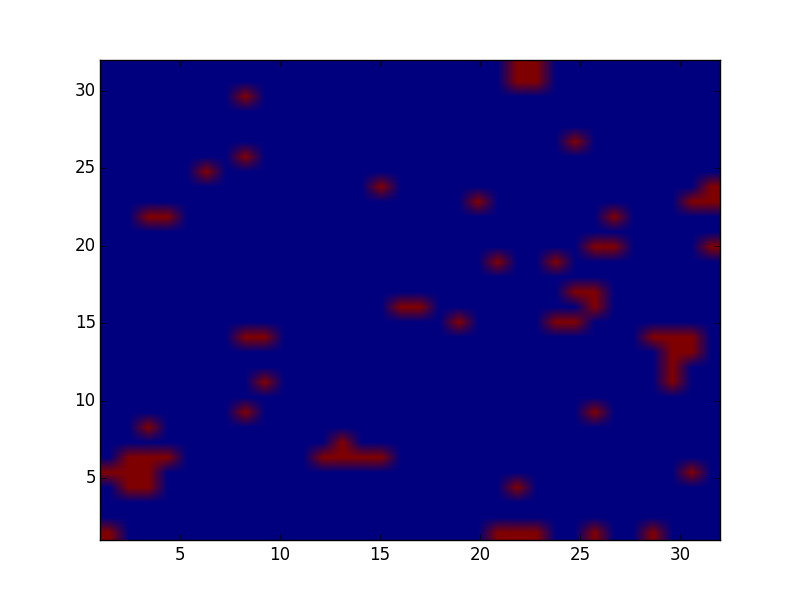
\includegraphics[scale=0.40]{2_run_3.png}
        \caption{Run 3, Random Initialization, converges to just above -1.0}
	    \label{fig:lat2_3}
    \end{subfigure}
    \caption{Plots drawn from lattice configurations after 700 iterations for T = 2.1 (Blue = -1, Red = +1 Magnetization)}
\end{figure}
Since the object gets magnetized at equilibrium for T = 2.1, we observe that some simulation runs show the object to be positively magnetised ( more red ) and some negatively magnetised ( more blue ). The ground state with lattice initialized to -1 is seen at negatively magnetised in figure (3.a) above. 
\clearpage
\subsubsection{T = 3.5}
\begin{figure}[!htb]
    \begin{subfigure}[b]{0.5\textwidth}
	    \centering
        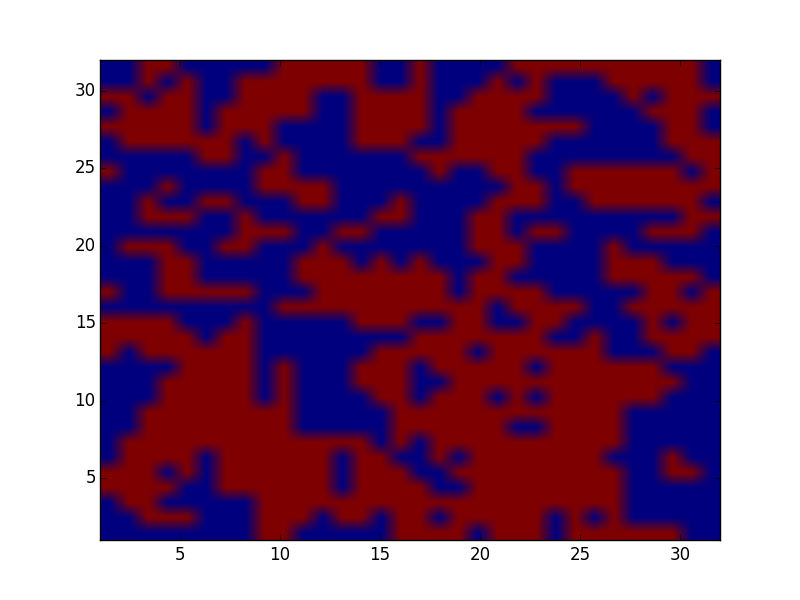
\includegraphics[scale=0.40]{3_run_0.png}
        \caption{Run 0, lattice initialized to -1, and simulations converges to ~ 0 magnetization}
	    \label{fig:lat3_0}
    \end{subfigure}
    \begin{subfigure}[b]{0.5\textwidth}
        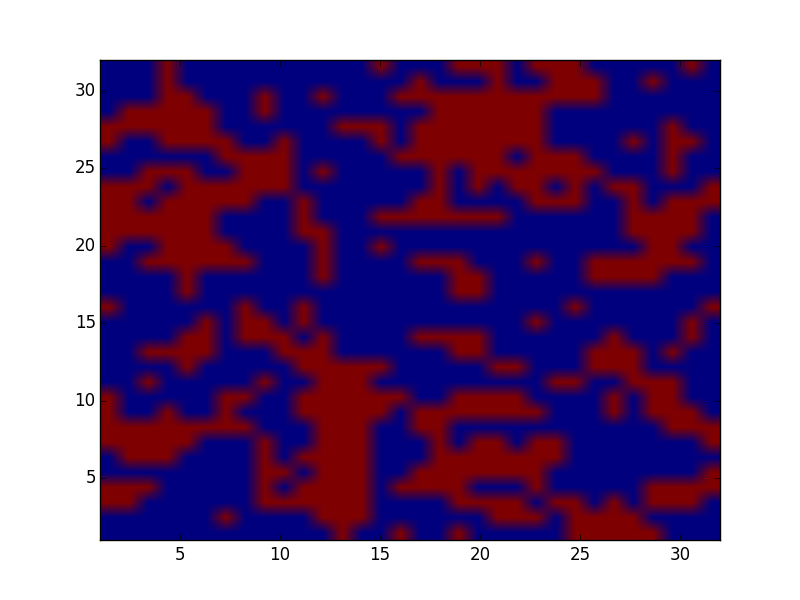
\includegraphics[scale=0.40]{3_run_2.png}
        \caption{Run 2, Random Initialization, stays at ~ 0.0 magnetization}
	    \label{fig:lat3_2}
    \end{subfigure}
    \caption{Plots drawn from lattice configurations after 700 iterations for T = 3.5 (Blue = -1, Red = +1 Magnetization)}
\end{figure}
At T = 3.5 since the object attains paramagnetism, it is seen to have almost equal patches of positive and negative magnetisation rendering the overall magnetisation close to zero. This is observed also for the ground state ( lattice initialized to -1 ) seen in figure (4.a) above.
\subsubsection{T = 2.265}
\begin{figure}[!htb]
	\centering
    \includegraphics[scale=0.40]{pics/50000_lattice.png}
    \caption{Lattice of T = 2.265 when convergence is just above -1.0. This plot from drawn from a configuration after 50,000 MCS (Blue = -1, Red = +1 Magnetization)}
	\label{fig:lat5k}
\end{figure}
At T = 2.265 since the object is going through phase transition, it is seen to exhibit either positive or negative magnetization for extended periods of time. This lattice visualization shows the object to have -ve magnetization after 50,000 MCS.
The corresponding python code can be found at \ref{code:problem1}
\clearpage
\subsection{Values of Averages}\label{prob2}
% $\langle m \rangle$ = \\
% $\langle \left|m\right|  \rangle$ = \\
In the table below we see that, at \\ \\
Temperature = 2.1 the mean magnetization is -ve but close to zero, that's expected, since 4 runs have converged to -1 and only 2 to +1 so they don't quite cancell out each other. The mean of the absolute magnetizations is quite close to 1 which is also inline with the theoretical result, that at equilibrium the magnetizations converge to -1 or +1 for temperatures below critical temperature.\\ \\
For Temperature = 3.5, the mean magnetization is quite close to zero and so is the mean of the absolute magnetization, these are again inline with theoretical results, according to which, for temperatures above critical temperature, the spins are disordered resulting in a mean magnetization which is close to zero.\\ \\
For Temperature = 2.265, the critical temperature, the magnetization keeps flipping between -1 and +1 so depending on our simulation run, we would get the mean slightly above zero or below zero because some +ve and -ve values in the sequence would cancell and the remaining values would get divided by the number of measurements which is quite large. Also the mean of absolute magnetizations is close to 0.75 because most of the values are between |0.5| and |1| (as can be seen in the 1.3) so the mean of them should be around 0.75 and our result is quite close to that. If we take longer runs, the value of <|m|> should converge to 0.75   

\begin{lstlisting}[caption=Average magnetization values]
For Temp = 2.1 <m> = -0.298180989583 err = 0.0149983573735 AND <|m|> = 0.872975260417 err = 0.000696132850481
For Temp = 3.5 <m> = 0.00534993489583 err = 0.00114563542299 AND <|m|> = 0.0633504231771 err = 0.00069438550247
For Temp = 2.265 <m> = -0.272830034722 err = 0.00295765007233 AND <|m|> = 0.659539149306 err = 0.000857419301299
\end{lstlisting}
The table above reports average M = $\langle m \rangle$ and average abs(M) = $\langle \left|m\right| \rangle$ values separately for each temperature. (magnetisation values have been taken from each run as follows):\\
For T = 2.1 : Equilibriation time is taken as 500\\
For T = 3.5 : Equilibriation time is taken as 200\\
For T = 2.265 : Equilibriation time is taken as 5000\\ \\
\textbf{Mean magnetisation} $\langle m \rangle$ is calculated by taking a mean of magnetisation values after equilibriation time for all run.\\
\textbf{Mean abs magnetisation} $\langle \left|m\right| \rangle$ is calculated by taking a mean of absolute values of magnetisation after equilibriation time for all run.\\
\textbf{Error values} are calculated using the following equation.\\
\begin{equation}
    \sigma_{m} = \sqrt{\frac{1}{n-1}(\langle m^{2} \rangle - \langle m \rangle^{2})}
\end{equation}


The corresponding python code can be found at \ref{code:problem2}
\subsubsection{The data below has mean values from each run of T=2.1 and T=3.5 (Raw data for reference ONLY)}
The below tables report average M = $\langle m \rangle$ and average abs(M) = $\langle \left|m\right| \rangle$ values separately for each run. \\
The averages were calculated by taking magnetization values from the past 100 MCS and averaging them to get average M. The average of the absolute values was calculated to get the average abs(M).\\
The \textbf{convergence criteria} was for the error ( difference between two successive averages ) to be less than 0.01
\begin{lstlisting}[caption=Average Magnetization values for T 2.1]
# Lattice initialized to -1 and then MC simulations were run
Temp = 2.1 Run 0 Convergence after 200 MCS at M = -0.876015625, M_err = 0.00283203125
Temp = 2.1 Run 0 Convergence after 200 MCS at abs(M) = 0.876015625, abs(M)err = 0.00283203125
Temp = 2.1 Run 0 Final Data after 1000 MCS at abs(M) = 0.879296875, abs(M)err = 0.0109765625, abs(M) = 0.879296875, abs(M)err = 0.0109765625

Temp = 2.1 Run 1 Convergence after 700 MCS at M = -0.89130859375, M_err = 0.0034765625
Temp = 2.1 Run 1 Convergence after 700 MCS at abs(M) = 0.89130859375, abs(M)err = 0.0034765625
Temp = 2.1 Run 1 Final Data after 1000 MCS at abs(M) = 0.90140625, abs(M)err = 0.02017578125, abs(M) = 0.90140625, abs(M)err = 0.02017578125

Temp = 2.1 Run 2 Convergence after 600 MCS at M = 0.884375, M_err = 0.00033203125
Temp = 2.1 Run 2 Convergence after 600 MCS at abs(M) = 0.884375, abs(M)err = 0.00033203125
Temp = 2.1 Run 2 Final Data after 1000 MCS at abs(M) = 0.84498046875, abs(M)err = 0.02615234375, abs(M) = 0.84498046875, abs(M)err = 0.02615234375

Temp = 2.1 Run 3 Convergence after 800 MCS at M = -0.885546875, M_err = 0.00876953125
Temp = 2.1 Run 3 Convergence after 800 MCS at abs(M) = 0.885546875, abs(M)err = 0.00876953125
Temp = 2.1 Run 3 Final Data after 1000 MCS at abs(M) = 0.886640625, abs(M)err = 0.0027734375, abs(M) = 0.886640625, abs(M)err = 0.0027734375

Temp = 2.1 Run 4 Convergence after 600 MCS at M = -0.8751171875, M_err = 0.00986328125
Temp = 2.1 Run 4 Convergence after 600 MCS at abs(M) = 0.8751171875, abs(M)err = 0.00986328125
Temp = 2.1 Run 4 Final Data after 1000 MCS at abs(M) = 0.88275390625, abs(M)err = 0.00666015625, abs(M) = 0.88275390625, abs(M)err = 0.00666015625

# Run 5 did not satisfy convergence criteria even after 1000 MCS
Temp = 2.1 Run 5 Final Data after 1000 MCS at abs(M) = 0.86546875, abs(M)err = 0.012421875, abs(M) = 0.86546875, abs(M)err = 0.012421875

Temp = 2.1 Run 6 Convergence after 800 MCS at M = -0.87662109375, M_err = 0.00427734375
Temp = 2.1 Run 6 Convergence after 800 MCS at abs(M) = 0.87662109375, abs(M)err = 0.00427734375
Temp = 2.1 Run 6 Final Data after 1000 MCS at abs(M) = 0.87595703125, abs(M)err = 0.026640625, abs(M) = 0.87595703125, abs(M)err = 0.026640625
\end{lstlisting}
\begin{lstlisting}[caption=Average Magnetization values for T 3.5]
# Lattice initialized to -1 and then MC simulations were run
Temp = 3.5 Run 0 Convergence after 300 MCS at abs(M) = 0.05380859375, abs(M)err = 0.0001171875
Temp = 3.5 Run 0 Convergence after 600 MCS at M = -0.03533203125, M_err = 0.008359375
Temp = 3.5 Run 0 Final Data after 1000 MCS at abs(M) = 0.053984375, abs(M)err = 0.01162109375, abs(M) = 0.053984375, abs(M)err = 0.01162109375

Temp = 3.5 Run 1 Convergence after 100 MCS at M = 0.02720703125, M_err = 0.00447265625
Temp = 3.5 Run 1 Convergence after 300 MCS at abs(M) = 0.05716796875, abs(M)err = 0.009609375
Temp = 3.5 Run 1 Final Data after 1000 MCS at abs(M) = 0.08421875, abs(M)err = 0.0171484375, abs(M) = 0.08421875, abs(M)err = 0.0171484375

Temp = 3.5 Run 2 Convergence after 700 MCS at abs(M) = 0.06861328125, abs(M)err = 0.0042578125
Temp = 3.5 Run 2 Final Data after 1000 MCS at abs(M) = 0.05421875, abs(M)err = 0.03365234375, abs(M) = 0.05421875, abs(M)err = 0.03365234375

Temp = 3.5 Run 3 Convergence after 100 MCS at M = 0.0115625, M_err = 0.0028125
Temp = 3.5 Run 3 Convergence after 200 MCS at abs(M) = 0.06232421875, abs(M)err = 0.00533203125
Temp = 3.5 Run 3 Final Data after 1000 MCS at abs(M) = 0.058125, abs(M)err = 0.00541015625, abs(M) = 0.058125, abs(M)err = 0.00541015625

Temp = 3.5 Run 4 Convergence after 400 MCS at abs(M) = 0.0665234375, abs(M)err = 0.0051953125
Temp = 3.5 Run 4 Final Data after 1000 MCS at abs(M) = 0.05048828125, abs(M)err = 0.013203125, abs(M) = 0.05048828125, abs(M)err = 0.013203125

Temp = 3.5 Run 5 Convergence after 100 MCS at abs(M) = 0.0578515625, abs(M)err = 0.00736328125
Temp = 3.5 Run 5 Final Data after 1000 MCS at abs(M) = 0.0575, abs(M)err = 0.0240625, abs(M) = 0.0575, abs(M)err = 0.0240625

Temp = 3.5 Run 6 Convergence after 500 MCS at M = 0.0059375, M_err = 0.00458984375
Temp = 3.5 Run 6 Convergence after 500 MCS at abs(M) = 0.0428125, abs(M)err = 0.00302734375
Temp = 3.5 Run 6 Final Data after 1000 MCS at abs(M) = 0.07537109375, abs(M)err = 0.02443359375, abs(M) = 0.07537109375, abs(M)err = 0.02443359375
\end{lstlisting}
\clearpage
\section{Appendix A}\label{code:problem1}
Python source code for \ref{prob1}.
\lstinputlisting{2d_example.py}
\section{Appendix B}\label{code:problem2}
Python source code for calculating means. \ref{prob2}
\lstinputlisting{2d_means.py}
\end{document}

   

